\documentclass{article}

\usepackage{amsmath}
\usepackage{graphicx}
\usepackage{float}
\usepackage{hyperref}
\usepackage{xcolor}
\usepackage{subfig}
\usepackage{natbib,url}
\usepackage[margin = 1in]{geometry}
\bibliographystyle{abbrv}

\def\epo{\epsilon\rightarrow 0}
\def\lb{\left(}
\def\rb{\right)}
\def\ls{\left[ \vphantom]}
\def\rs{\right] }
\def\ep{\epsilon}

\title{Conjugate heat transfer in Icy Moons}
\author{Tobias Oliver}
\date{}

\begin{document}
\maketitle
\section{Summary}
\section{Intellectual Merit}
The solar system contains a number of icy bodies, many of which are thought to be ``ocean worlds,'' that may be suitable candidates for the habitability of life.
The primary objective of NASA's \textit{Europa Clipper} (EC) (eg.\citep{pC14_JUICE}) and ESA's \textit{Jupiter Icy Moons Explorer} (JUICE)\citep{oG13} missions is to investigate Europa, Ganymede, and Callisto, three Jovian satellites believed to be ocean worlds. Each is expected contain salty, liquid oceans underneath thin icy shells \citep{rP99,fN16}, and both EC and JUICE aim to determine whether these bodies contain necessary conditions for life\citep{tB24}.
The sub-surface oceans link the solid cores of these moons to their icy exteriors, and are therefore expected to play an important role in the transport of heat and chemicals to their surfaces \citep{kS20}. 

The dynamics of these oceans are poorly understood, and neither EC nor JUICE will be able to make direct observations of the oceans. 
Therefore, forward numerical simulations are necessary to understand the interior dynamics. 
Furthermore, the coupling processes between the ocean and icy surface needs to be studied in order to make predictions that can be verified by the upcoming missions.
Current constraints on the thickness of Europa's ice shell, for example, range between $5-30$ km \citep{sV18}, but EC is expected to significantly reduce this uncertainty as well as provide spatially varying temperature profiles of the surface \citep{kS20}. 
Observations such as these will hint at the ocean dynamics, but only through processes not currently understood. In order to make the best use of EC and JUICE, it is necessary to have models that allow us to extrapolate surface measurements down to the oceans.
Indeed, a better understanding of coupled ice-ocean studies is one of the key future issues outlined in the most recent review of icy moon oceanography \citep{kS24}. 

The proposed project would investigate forward, hydrodynamical models in which the coupling between the liquid ocean and icy surface is included. Two different coupling mechanisms will be studied. 
First, a conjugate heat transfer (CHT) model, in which the time-varying temperature profile in the icy shell is solved, will be built and run, which will provide new insight into the surface response to the underlying convection. Second, the double diffusion process, in which the bouyancy effects of both temperature and salinity are accounted for, will be investigated in the context of the ice-ocean boundary. Both studies will use 3D forward models of rotating convection in full spherical shells. 
\section{Background}
Europa, Callisto, and Ganymede, as well as the Saturnian moons Enceladus and Triton, were identified as likely ocean worlds after data started returning from the \textit{Galileo} and \textit{Cassini} missions \citep{fN16}.
Both gravity and magnetic measurements aided in the discovery, but in the case of Europa, the latter proves more convincing. 
Since the magnetic dipole of Jupiter is tilted about $10^{\circ}$ with respect to the orbital plane, the Jovian moons experience a magnetic induction as they orbit the planet.
Induced magnetic fields were measured by \textit{Galileo}, and it has been determined that a conducting ocean near the surface is likely necessary to explain the measurements \citep{fN16,cZ00}. 

A variety of forcing mechanisms have been proposed and discussed, and it is likely that the oceans are turbulent and capable of convecting a large amount of heat and chemicals between the solid interior and icy crust.
These mechanisms include electromagnetic coupling between the conducting ocean and the Jovian magnetic field \citep{cGlP19} and a variety of mechanical effects such as tides and precession \citep{kS24}. 
Here I propose to study buoyantly driven flows, in which variations in the fluid density drive convection.
Density are usually attributed to two separate effects-- thermal and compositional heterogeneities.
Thermally driven flows can be driven by radiogenic heating from the silicate core \citep{kS14,kS19,jK22} or tidal heating \citep{gT03,dL23}, which results in heterogeneous thermal forcing and may explain lateral variations in ice shell thickness. 
Compositional buoyancy is usually discussed in the context of salt fluxes near the outer boundary. 
Freezing (melting) can increase (decrease) salinity. The associates density variations drives convection and References \citep{yA21,wK22} predict that this mechanism serves to flatten the ice shell of Europa (ie.  homogenous thickness). 

From a forward modeling perspective, the largest challenge we face is the disparity between the spatial and temporal scales relevant to geophysical bodies, and the scales that we can realistically simulate. We usually formalize this issue in terms of non-dimensional numbers that reflect the range of scales in the physical problem. Alterntively, we can think of these quantities as ratios of different forcing terms in the governing equations. 
In a geophysical and astrophysical context, there are two non-dimensional numbers of particular importance: the Rayleigh and Ekman numbers. The Rayleigh number $Ra$ describes the ratio of buoyancy to diffusivity. For planetary bodies, $Ra$ is very large, generally indicating vigourous convection.
The Ekman number $Ek$ approximates the ratio of viscous diffusion to Coriolis effects associated with the rotation of the planet. Due to the large spatial scales, values for $Ek$ tend to be very small, indicating that rotation plays a dominant role.
The Nusselt number $Nu$ is the ratio of total heat transfer to conductive heat transfer and is greater than $1$ for convective problems. The Prandtl number $Pr$ is the ratio of thermal to momentum diffusivity and is beleived to be $O\lb 10\rb $ for the icy moons \citep{kS24}.
The definition for these quantities are
\[Ra = \frac{g\alpha\Delta T D^{3}}{\nu\kappa}\;\;\;Ek = \frac{\nu}{D^{2}\Omega}\;\;\; Pr = \frac{\nu}{\kappa}\;\;\; Nu = \frac{hD}{k},\]
where $g$ is the surface gravitational acceleration, $\alpha$ is the coefficient of thermal expansion, $D$ is the ocean thickness, $\nu$ and $\kappa$ are the diffusivities of momentum and temperature respectively, $\Omega$ is the planetary rotation rate, $h$ is the total heat transfer, and $k$ is the thermal conductivity. $\Delta T$ indicates the temperature between the ocean surface and floor.
A related value $Ra_{s}$ for compositional convection can be defined in a similar manner by replacing the appropriate values for $\alpha,\kappa,$ and $\Delta T.$
To take Europa as an example, predicted values of $Ra$ and  $Ek$ are $O\lb 10^{20}\rb $ and $O\lb 10^{-12}\rb $ respectively, however modern direct numerical simulations (DNS) have only reached values of $Ra \sim 10^{8}$ and $Ek \sim 10^{-5}.$ \citep{dL23}. In a broader geophysical context, more aggressive simulations have been performed \textcolor{red}{token citations \citep{cG19}}, however all fall significantly short of reaching the target values. For icy moons, it is particularly difficult to reach small values of $Ek$ because the ocean depth is much smaller than the planetary radius. As such, the usual procedure is to attempt to establish scaling laws with the non-dimensional parameters by simulating at moderate values, and then extrapolating to planetary values.
\begin{figure}
	\begin{center}
		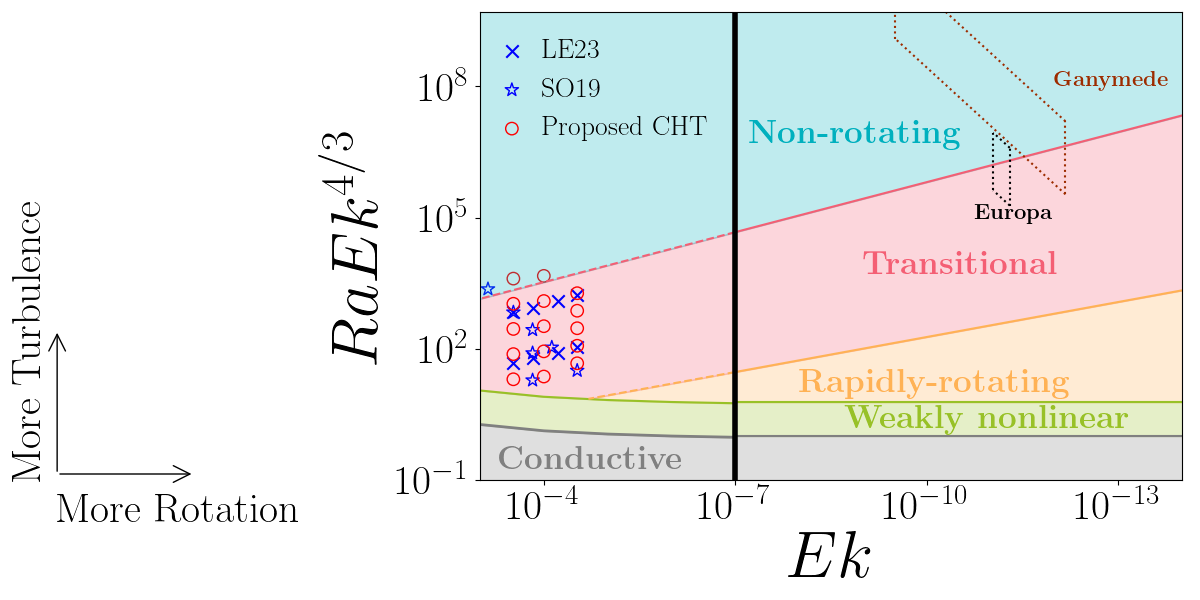
\includegraphics[width=0.6\textwidth]{figures/reg_diagram}
	\end{center}
	\caption{Regime diagram for rotating convection, adapted from \citep{dL23,tG16}. The region left of the solid black line represent DNS results at $Pr = 1$ for a Europa-like geometry\citep{aB22}. The region right of the black line represents scaling predictions from \citep{tG16}. Dashed lines represent extrapolations of asymptotic predictions into the DNS region. Crosses and stars give the parameter space of modern simulations from Lemasquerier et al. 2023\citep{dL23} and Soderlund 2019\citep{kS19} respectively. Regions enclosed by dotted lines represent approximate parameter space for Europa and Ganymede \citep{dL23,kS19}. Red markers indicate proposed simulations for conjugate heat transfer (CHT) study.}
	\label{f:reg_d}
\end{figure}

To further complicate matters, it is insufficient to establish scaling relations for each non-dimensional parameter independently, because the flow behaviours can vary wildly depending on the particular combination of the non-dimensional parameters. 
For example, at a value of $Ra = 10^{8}$ a non-rotating flow ($Ek\rightarrow \infty$) is expected to vigourously convect, however rapid rotation (low  $Ek$) will stifle and change the structure of the convection, or even arrest it entirely. 
Figure \ref{f:reg_d} displays a cross-section of $Ek,Ra$ parameter space, and the associated regimes. The ordinate has been rescaled by $Ek^{4/3}$ because for rotating flows the parameter $RaEk^{4/3}$ determines the boundary between conduction and convection \citep[e.g. ][]{sC61}.

For $RaEk^{4/3}<O\lb 1\rb,$  rotational effects dominate the system and supress radial motion. This regime is referred to as conductive, since all heat is transported conductively. As $Ra$ is increased, convection sets in as axially stretched flows conforming to the Taylor-Proudman theorem \citep{gB53}, which dictates that rapidly-rotating flows remain invariant along the axis of rotation. Such dynamics are known as geostrophic.
Geostrophic flows are laminar over a small range of $Ra,$ but quickly become turbulent. Geostrophy holds over large time and length scales, but on small scales low order fluctuations make the dynamics highly non-linear.
This regime is often referred to as ``rapidly rotating'' or ``geostrophic turbulence'' \citep{kJ12}.
Further increase of $Ra$ yields the ``transitional" regime, where geostrophy no longer holds, but flows are still rotationally influenced.
Although significant uncertainty exists, it is believed that for the Jovian ocean worlds the primary regime of interest is the Transitional regime, in which rotation, buoyancy, and pressure play leading order roles \citep{dL23,tG16}.

Most studies \citep{kS19, dL23} have investigated only the ocean domain, and have prescribed boundary conditions at the ocean-ice interface to represent the fixed melting temperature of the ice. 
A model with a dynamic, melting icy boundary has been studied, however the authors were primarily interested in the resulting topography. The fast timescale heat fluctuations in the icy shell due to the underlying convection were not investigated \citep{jK24}. 

CHT is a simulation configuration in which a solid boundary is included in the solution domain so that heat is able to conduct from the fluid into the boundary. Rather than placing a boundary condition on the fluid surface, the condition is placed on the outermost solid surface and the interface is solved \citep{dA09}. The significance of this effect can be estimated by the value of the Biot number $Bi$ \citep{dA09,jL24}, a non-dimensional parameter respresenting the ratio of conductive resistance to convective heat flow. For the conjugate problem, $Bi$ can be estimated as
\[Bi \sim Nu\frac{k_{f}}{k_{i}}\frac{D_{i}}{D_{f}},\]
where $k_{f\lb i\rb }$ is the thermal conductivity of the fluid (ice) and $D_{f\lb i\rb }$ is the fluid (ice) depth.
Estimates for Europa therefore suggest $Bi \sim O\lb 10^{6}\rb$ \citep{dL23}. When $Bi>1,$ the conjugate problem is considered relevant, and therefore this process likely plays a role in the evolution of icy shells.
\subsection{Compositional convection}
On Earth, solutal composition is known to play a dominant role in oceanic convection \textcolor{red}{indicate you know what you're talking about....} The electrical conductive properties of the Jovian satellites likely imply salty oceans\citep{cZ00}, which suggests a variety of consequences. At pressures relevant to the icy moons, salinity can reverse the sign of the thermal expansivity coefficient $\alpha$ at temperatures close to, but greater than, the melting temperature. This means that colder fluid is less dense, which may allow for the generation of a buoyantly stable layer that inhibits heat and mass transport \citep{aT64}. 
Furthermore, salinity affects fluid density even in the absence of temperature variations. This mechanism provides a second source of buoyancy and can yield double diffusive convection.
\section{Proposed project and methodology}
I propose to sets of simulations in order to study ice-ocean coupling in the icy moons.
\subsection{Conjugate heat transfer}
\begin{table}
\begin{center}
\begin{tabular}{|c|c|c|}
\hline
$Ra$&$Ek$&$D_{f}/D_{i}$\\
\hline
$\lb 5 \times 10^{6} - 2 \times 10^{8} \rb $ & $3 \times 10^{-4} $ & $2,10$\\
\hline
$\lb 5 \times 10^{6} - 1 \times 10^{9} \rb $ & $1 \times 10^{-5} $ & $2,10$\\
\hline
$\lb 5 \times 10^{7} - 2 \times 10^{9} \rb $ & $3 \times 10^{-5} $ & $2,10$\\
\hline
\end{tabular}
\end{center}
\caption{Proposed parameter space}
\label{t:param}
\end{table}
I will explore Boussinesq convection in a thin, liquid shell surrounded by a thermally conducting layer. 
In particular, I will perform a sweep of $30$ simulations across parameter space (see table \ref{t:param}, figure \ref{f:reg_d}) and extrapolate the results to regimes associated with icy moons.
At larger values of $Ek,$ I will simulate the transitional and non-rotating regimes, however at the smallest $Ek$ values, I intend to focus on the transitional regime in order to better compare with existing studies and reduce computational cost.
The hydrodynamic code \texttt{Nek5000}\citep{nek5000} is capable of solving the CHT problem and I have already used the code extensively to solve related geophysical problems. 
Based on the numerical resolutions reported in \citep{dL23}, I estimate that $3\times 10^{6}$ CPU-hours will be necessary to complete these simulations.

Primarily, I will report temperature distributions within the icy shell. I will also investigate global transport quantites, such as convected heat, and structural quantities, such as latitudinal profiles of temperature. 
These latter results can be compared to existing studies \citep[e.g.][]{dL23,kS19,jK22} to determine whether the CHT setup has significant effects on the convection itself.
\subsection{Solutal convection}
I will also investigate double-diffusive convection in a non-rotating and slowly rotating (moderate $Ek$) context. Due to the significant computational constraints, I propose to study a shperical shell geometry for only non-rotating and slowly rotating ($Ek = 10^{-4}$) flows. I will suplement these results with a suite of local, rotating simulations in cartesian plane layers.

\small
\bibliography{References,journal_abbreviations}%jfm-bib,References}
\end{document}
